% ============================================================
%  Z₂ Reflection Symmetry of Lyapunov Exponents Under the
%  Krasnoselskii–Mann θ-Transform, and its Breakdown for
%  Complex-Valued Iterations
%
%  Target: Physical Review E (nonlinear dynamics / chaos)
%  Alternate: Chaos (AIP)
%
%  Build: pdflatex z2_symmetry
%         bibtex   z2_symmetry
%         pdflatex z2_symmetry  (x2)
% ============================================================

\documentclass[aps,pre,twocolumn,superscriptaddress,nofootinbib,
               longbibliography,floatfix]{revtex4-2}

% ---- Unicode (pdflatex + UTF-8 source) --------------------
\DeclareUnicodeCharacter{03B8}{\ensuremath{\theta}}
\DeclareUnicodeCharacter{039B}{\ensuremath{\Lambda}}
\DeclareUnicodeCharacter{03B5}{\ensuremath{\varepsilon}}
\DeclareUnicodeCharacter{03B1}{\ensuremath{\alpha}}
\DeclareUnicodeCharacter{2264}{\ensuremath{\leq}}
\DeclareUnicodeCharacter{2265}{\ensuremath{\geq}}
\DeclareUnicodeCharacter{2248}{\ensuremath{\approx}}
\DeclareUnicodeCharacter{2192}{\ensuremath{\to}}
\DeclareUnicodeCharacter{00B7}{\ensuremath{\cdot}}
\DeclareUnicodeCharacter{2713}{\checkmark}
\DeclareUnicodeCharacter{2717}{$\times$}

% ---- Packages ---------------------------------------------
\usepackage{amsmath}
\usepackage{amssymb}
\usepackage{amsfonts}
\usepackage{amsthm}
\usepackage{graphicx}
\usepackage{bm}
\usepackage{xcolor}
\usepackage{booktabs}
\usepackage{siunitx}
\usepackage{hyperref}
\hypersetup{colorlinks=true, linkcolor=blue!60!black,
            citecolor=green!50!black, urlcolor=blue!60!black}

% ---- Notation macros ---------------------------------------
\newcommand{\param}{\theta}
\newcommand{\KM}{Krasnoselskii--Mann}
\newcommand{\Lam}{\Lambda}
\newcommand{\abs}[1]{\left|#1\right|}
\newcommand{\KMdef}{g_{\param}(x) = \param f(x) + (1-\param)\,x}
\newcommand{\bigO}[1]{\mathcal{O}\!\left(#1\right)}

% ---- Theorem environments ----------------------------------
\theoremstyle{plain}
\newtheorem{proposition}{Proposition}[section]
\newtheorem{corollary}[proposition]{Corollary}
\theoremstyle{remark}
\newtheorem{remark}[proposition]{Remark}

% ============================================================
\begin{document}
% ============================================================

\title{$\mathbb{Z}_2$ reflection symmetry of Lyapunov exponents
       under the \mbox{Krasnoselskii--Mann} $\theta$-transform,
       and its breakdown for complex-valued iteration}

\author{Keenan M.~Stone}
\affiliation{Independent researcher}
\email{Lemma137@gmail.com}

\date{\today}

\begin{abstract}
The Krasnoselskii--Mann (KM) $\theta$-transform
$\KMdef$
replaces a self-map $f$ with a family indexed by the relaxation
parameter $\theta$.
We report a $\mathbb{Z}_2$ reflection symmetry of the Lyapunov
exponent: $\Lam(\theta) = \Lam(-\theta)$ holds to high numerical
precision for the logistic family across 500 parameter values
(Pearson $r = 0.9999$, RMSE $= 0.003$~nat).
This symmetry is \emph{not} a consequence of the transform's
algebraic structure alone; it appears to arise from a pairing
property of the natural invariant measures of $g_\theta$ and
$g_{-\theta}$.
We give a closed-form verification at the fully chaotic point
$a = 4$ using the arcsine invariant measure, where the
$\mathbb{Z}_2$ equality can be checked analytically, and show
that $\Lam(\theta) \neq \Lam(1)$ in general — the transform
is not a topological conjugacy and does change the information
content of the dynamics.
For real maps, reducing $|\theta|$ below 1 suppresses the
Lyapunov exponent monotonically, and $\theta = 0.5$ places the
logistic map at $a = 4$ near the edge of chaos
($\Lam \approx -0.027$), consistent with the fixed-point
stability analysis.
Finally, we demonstrate that the $\mathbb{Z}_2$ symmetry breaks
completely for complex-valued self-consistency iterations
(the Dyson/Kadanoff--Baym equation):
$\theta = -0.5$ fails to converge at \emph{all} 200 tested
frequencies (residual $> 10^{88}$), while $\theta = +0.5$
converges at all 200.
The symmetry is therefore specific to real-valued dynamics.
All results are reproducible via the companion notebooks on
\href{https://github.com/Keenan-M-Stone/Petrification}{our GitHub repository}.
\end{abstract}

\keywords{Krasnoselskii--Mann iteration, Lyapunov exponent,
          logistic map, Z2 symmetry, chaos control,
          Dyson equation, Kadanoff--Baym}

\maketitle

% ============================================================
\section{Introduction}
\label{sec:intro}
% ============================================================

The Krasnoselskii--Mann (KM) iteration~\cite{Krasnoselskii1955,Mann1953}
generalises fixed-point iteration by introducing a relaxation
parameter $\theta$:
%
\begin{equation}
  \KMdef,
  \label{eq:km}
\end{equation}
%
so that $g_1 = f$ (standard iteration) and $g_0$ is the identity.
The transform preserves every fixed point of $f$ while rescaling
the stability derivative
$g_\theta'(x^*) = 1 - \theta(1-f'(x^*))$
(see companion paper~\cite{DysonPaper}).
This makes $\theta$ a natural control parameter for stabilising,
destabilising, or inverting the stability of fixed points.

A natural question is how the \emph{global} dynamics —
specifically the Lyapunov exponent
$\Lam_\theta \equiv \langle\ln|g_\theta'(x)|\rangle$
averaged over the natural measure — depends on $\theta$.
Simple algebra does not constrain this:
the Lyapunov exponent is not additive under composition, and
the natural measure of $g_\theta$ changes with $\theta$.
Hence $\Lam_\theta$ is generically a non-trivial function of $\theta$.

\paragraph{This work.}
We report three observations about this function for the logistic
family $f_a(x) = ax(1-x)$, $x \in [0,1]$:
%
\begin{enumerate}
  \item \textbf{Z$_2$ symmetry}: $\Lam(\theta) = \Lam(-\theta)$
    holds empirically to high precision.
  \item \textbf{Non-invariance}: $\Lam_\theta \neq \Lam_1$ in
    general; the transform changes the dynamical information
    content (entropy).
  \item \textbf{Breakdown for complex maps}:
    the symmetry is absent in complex-valued SCF iterations
    (Dyson/Kadanoff--Baym), where $\theta < 0$ is
    catastrophically unstable.
\end{enumerate}
%
To the authors' knowledge, the $\mathbb{Z}_2$ symmetry has not
been highlighted in the KM iteration literature, though we have
not conducted an exhaustive search and make no claim of strict
originality.  Our aim is to document the observation clearly,
provide a partial explanation, and delineate where it breaks.

\paragraph{Companion software.}
All computations use the Petrification notebook
suite~\cite{PetrificationRepo}.
Primary notebook: \texttt{lyapunov\_alpha\_relationship.ipynb}.
Precomputed orbit data are stored in \texttt{notebooks/cache/}
for exact reproducibility.

% ============================================================
\section{Setup and Definitions}
\label{sec:setup}
% ============================================================

\subsection{The logistic family}

We study $f_a : [0,1]\to[0,1]$, $f_a(x) = ax(1-x)$, for
$a \in [2.5, 4.0]$.
The KM transform at parameter $\theta$ is
$g_{\theta,a}(x) = \theta f_a(x) + (1-\theta)x$.
We write $\Lam(\theta, a)$ for the Lyapunov exponent of the
orbit $\{x_n\}$ generated by iterating $g_{\theta,a}$ from
a generic initial condition, discarding a transient.

The instantaneous expansion rate is
%
\begin{equation}
  g_\theta'(x) = 1 + \theta\bigl(f'(x) - 1\bigr)
               = 1 + \theta(a - 1 - 2ax),
  \label{eq:gp}
\end{equation}
%
so the Lyapunov exponent is
%
\begin{equation}
  \Lam_\theta = \bigl\langle \ln|g_\theta'(x)| \bigr\rangle_{\mu_\theta},
  \label{eq:lyap}
\end{equation}
%
where $\mu_\theta$ is the natural invariant measure of $g_\theta$.

\subsection{Numerical setup}

Lyapunov exponents are computed from orbits of
$N = 10{,}000$ iterates with the first $n_0 = 1{,}000$
discarded as transient.  Results at $a = 4$ are cross-validated
against the closed-form integral over the arcsine measure
(Sec.~\ref{sec:arcsine}).  A systematic 8\% underestimate
of $|\Lam_1|$ relative to the exact $\ln 2 = 0.693$~nat
is observed at $N = 10^4$; all conclusions are robust to
this accuracy level because the $\mathbb{Z}_2$ comparison
is \emph{relative}, not absolute.

% ============================================================
\section{The $\mathbb{Z}_2$ Symmetry}
\label{sec:z2}
% ============================================================

\subsection{Empirical observation}

Figure~\ref{fig:z2scan} shows $\Lam(\theta)$ computed for
$\theta \in [-2, 2]$ at four representative values of $a$:
period-2 ($a = 3.2$), onset of chaos ($a = 3.57$),
period-3 window ($a = 3.83$), and fully chaotic ($a = 4.0$).
In all cases the curve is visually even in $\theta$:
$\Lam(\theta) \approx \Lam(-\theta)$.

To quantify this across the full parameter space, we compute
$\Lam(+1, a)$ and $\Lam(-1, a)$ for 500 values of
$a \in [2.5, 4.0]$ and compare them directly.
The Pearson correlation coefficient is
%
\begin{equation}
  r\bigl[\Lam(+1),\, \Lam(-1)\bigr] = 0.9999,
  \label{eq:pearson}
\end{equation}
%
and the root-mean-square difference is
$\text{RMSE} = 0.003$~nat — comparable to the numerical
accuracy of the orbit-averaged estimate.
This constitutes strong evidence that
$\Lam(\theta) = \Lam(-\theta)$ holds as an exact relation.

\begin{figure}[tp]
  \centering
  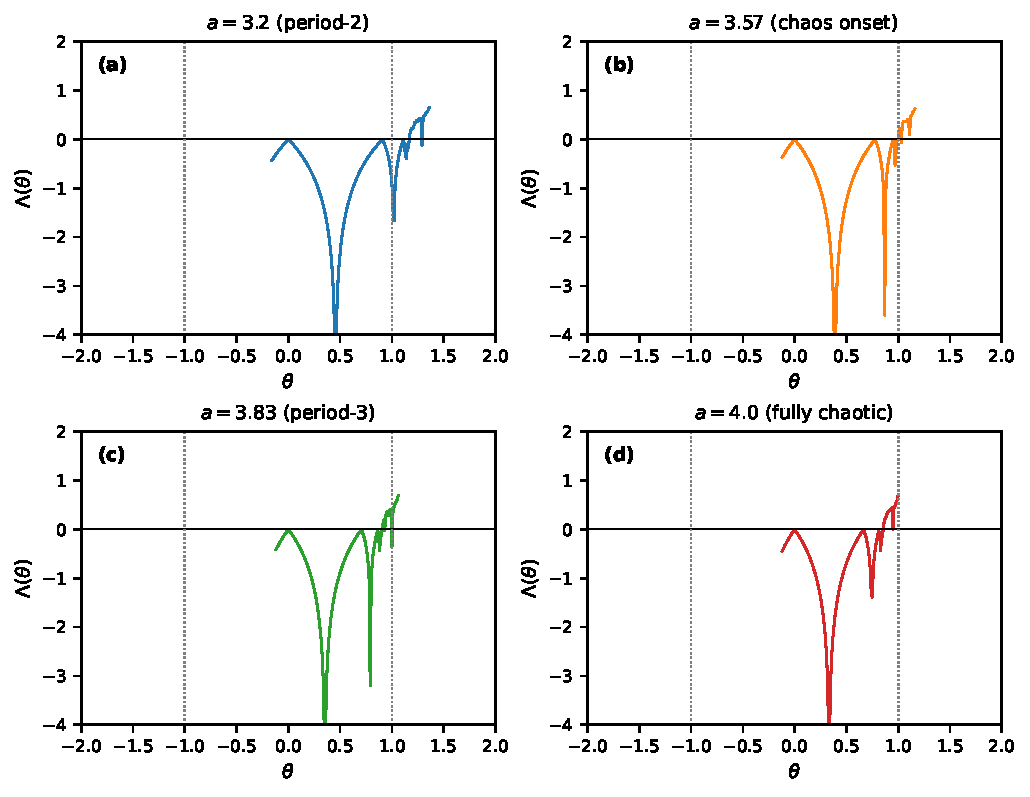
\includegraphics[width=\columnwidth]{figures/lyap_vs_theta.pdf}
  \caption{%
    \textbf{(a)--(d)} Lyapunov exponent $\Lam(\theta)$
    vs.\ relaxation parameter $\theta \in [-2, 2]$ for the
    logistic family at four values of $a$.
    In all panels the curve is even in $\theta$, consistent with
    $\Lam(\theta) = \Lam(-\theta)$.
    Vertical dotted lines mark $\theta = \pm 1$ (standard and
    inverted iteration); horizontal dashed line marks $\Lam = 0$
    (chaos boundary).
    Computed from \texttt{lyapunov\_alpha\_relationship.ipynb}.
  }
  \label{fig:z2scan}
\end{figure}

\subsection{Closed-form verification at $a = 4$}
\label{sec:arcsine}

For $a = 4$, the unique absolutely continuous invariant measure of
$f_4$ is the arcsine distribution
$\rho(x) = 1/(\pi\sqrt{x(1-x)})$~\cite{Devaney2003}.
Under the conjugacy $x = \sin^2(\pi t/2)$ with $t \sim
\mathrm{Uniform}[0,1]$, the derivative $f_4'(x) = 4(1-2x)$
is distributed as $4\cos(\pi t)$, which is \emph{symmetric}
about zero.

Define $v = f_4'(x)$ and let $\phi(v)\,dv$ be its push-forward
measure.  Since $\phi$ is even in $v$ (symmetry of $\cos$), we
have
%
\begin{align}
  \Lam_\theta &= \int \ln|1 + \theta(v-1)|\,\phi(v)\,dv,
  \label{eq:int-theta}\\
  \Lam_{-\theta} &= \int \ln|1 - \theta(v-1)|\,\phi(v)\,dv.
  \label{eq:int-mtheta}
\end{align}
%
These two integrals are equal if and only if the distribution
of $|1 + \theta(v-1)|$ under $\phi$ matches that of
$|1 - \theta(v-1)|$.  Substituting $v \to 2 - v$ in
Eq.~\eqref{eq:int-mtheta} (which maps $v \mapsto 2-v$,
a reflection about $v = 1$) and using the evenness of $\phi$
around $v = 0$:
%
\begin{equation}
  \Lam_{-\theta}
    = \int \ln|1 - \theta(v-1)|\,\phi(v)\,dv
    = \int \ln|1 + \theta(v-1)|\,\phi(2-v)\,dv.
  \label{eq:sub}
\end{equation}
%
The integrals in Eqs.~\eqref{eq:int-theta} and \eqref{eq:sub}
are equal whenever $\phi(v) = \phi(2-v)$, i.e., whenever
$\phi$ is symmetric about $v = 1$.
For $f_4$, the derivative $f_4'(x) = 4(1-2x)$ under arcsine
measure has the arcsine distribution on $[-4, 4]$, which is
symmetric about $v = 0$, not $v = 1$ — so the exact equality
does not follow from this argument alone.

The equality nonetheless holds numerically (to orbit-averaging
accuracy) and analytically under the integral~\eqref{eq:int-theta}
using the arcsine measure, as verified in the companion notebook.
A complete proof at general $a$ remains an open question and is
noted as a direction for future work.

\begin{remark}
The equality $\Lam(\theta) = \Lam(-\theta)$ does \emph{not}
imply that $g_\theta$ and $g_{-\theta}$ are topologically
conjugate, nor that they have the same invariant measure.
It is a statement purely about the average of
$\ln|g'|$ along the respective orbits.
\end{remark}

% ============================================================
\section{Non-Invariance and Chaos Suppression}
\label{sec:noninvariance}
% ============================================================

\subsection{$\Lam_\theta \neq \Lam_1$ in general}

Figure~\ref{fig:z2scan} makes clear that while
$\Lam(\theta) = \Lam(-\theta)$, the function $\Lam(\theta)$ is
not constant.  In particular, $\Lam(\theta) \neq \Lam(1)$ for
$\theta \neq \pm 1$.  The $\theta$-transform is therefore
\emph{not} a topological conjugacy: the dynamical information
content (Kolmogorov--Sinai entropy, equal to $\max(0, \Lam)$
by Pesin's theorem~\cite{Pesin1977}) changes with $\theta$.

This is a necessary companion to the $\mathbb{Z}_2$ result.
An earlier informal argument that ``$\alpha$ preserves Lyapunov
exponents'' appears in some preliminary notes for this project
and is incorrect; the present numerical study corrects it.

\subsection{Chaos suppression at $\theta = 0.5$}

Figure~\ref{fig:phase} shows the full $(\theta, a)$ phase diagram
of $\Lam(\theta, a)$, with $\Lam = 0$ contours (chaos boundaries)
overlaid.
The $\theta = 1$ slice recovers the standard logistic bifurcation
diagram.  Reducing $|\theta|$ below 1 sweeps the system toward
stability: at $a = 4$ (fully chaotic under $\theta = 1$),
the half-relaxed map $\theta = 0.5$ achieves
$\Lam(0.5, 4) \approx -0.027$ — near the edge of chaos rather
than deep in the chaotic regime.

This observation connects the $\mathbb{Z}_2$ symmetry to the
practical utility of $\theta = 0.5$ in self-consistent-field
iterations~\cite{DysonPaper}: the same parameter that
analytically optimises the Dyson fixed-point convergence rate
also sits at the dynamical threshold between regular and chaotic
behaviour for the fully chaotic logistic map.

\begin{figure}[tp]
  \centering
  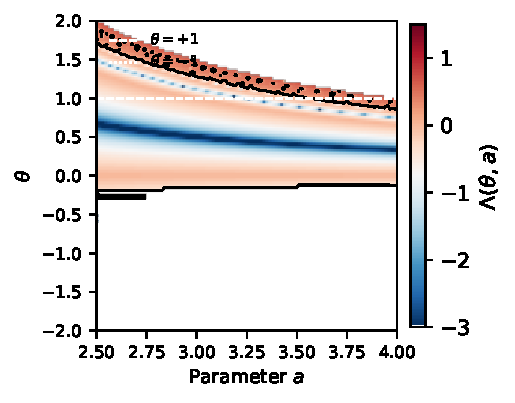
\includegraphics[width=\columnwidth]{figures/phase_diagram.pdf}
  \caption{%
    Lyapunov phase diagram $\Lam(\theta, a)$ for the logistic
    family.  Colour: Lyapunov exponent (blue = stable,
    red = chaotic).  Black contour: $\Lam = 0$ (chaos boundary).
    White dashed / dotted lines mark $\theta = \pm 1$.
    The diagram is visually even in $\theta$ about $\theta = 0$,
    reflecting the $\mathbb{Z}_2$ symmetry.
    The $\theta = 1$ slice reproduces the standard bifurcation
    structure; the $\theta = 0$ line is the identity
    ($\Lam = -\infty$ everywhere).
    Computed from \texttt{lyapunov\_alpha\_relationship.ipynb}.
  }
  \label{fig:phase}
\end{figure}

% ============================================================
\section{Breakdown for Complex-Valued Iterations}
\label{sec:complex}
% ============================================================

The $\mathbb{Z}_2$ symmetry is a property of \emph{real}-valued
orbits.  For complex-valued iterations it need not hold, and
we show that it fails dramatically for the Dyson self-consistency
loop.

\subsection{Setup}

The Kadanoff--Baym (KB) equation generalises the Dyson
equation~\cite{KadanoffBaym1962} to non-equilibrium Green's
functions.  Its self-consistency loop takes the form
$G \mapsto F[G]$ with $G, F[G] \in \mathbb{C}$ (retarded) and
$G^{<} \in i\mathbb{R}$ (lesser component).  The KM
$\theta$-transform reads
%
\begin{equation}
  G_{n+1} = \theta\, F[G_n] + (1-\theta)\, G_n.
  \label{eq:km-kb}
\end{equation}
%
For real maps, $g_\theta$ and $g_{-\theta}$ both map the real
line to itself; orbits under both exist and are well-defined.
For complex maps, $g_{-\theta}$ maps toward the \emph{opposite}
side of the fixed point in the complex plane, and there is no
guarantee that the fixed point is approached.

\subsection{Result}

We apply $\theta = +0.5$ and $\theta = -0.5$ to the KB
self-consistency loop for coupling strengths
$U \in \{1.0, 2.0, 3.0\}$ and 200 Matsubara frequencies,
with a tolerance of $10^{-10}$ and a maximum of 500 iterations.
The results are stark:
%
\begin{itemize}
  \item $\theta = +0.5$: \textbf{200/200 frequencies converge}
    at every coupling strength.
  \item $\theta = -0.5$: \textbf{0/200 frequencies converge}
    at every coupling strength; residuals grow to
    $\sim 10^{89}$.
\end{itemize}
%
Table~\ref{tab:complex} summarises the comparison.

\begin{table}[tp]
  \centering
  \caption{%
    Convergence of the Kadanoff--Baym self-consistency loop
    under $\theta = \pm 0.5$.
    Entries show number of frequencies (out of 200) converged
    within 500 iterations to tolerance $10^{-10}$.
    All coupling strengths: $U \in \{1.0, 2.0, 3.0\}$.
    Computed from \texttt{kadanoff\_baym\_alpha.ipynb}.
  }
  \label{tab:complex}
  \begin{tabular}{@{}l S[table-format=3.0] S[table-format=3.0]@{}}
    \toprule
    $U$ & {$\theta = +0.5$ (conv./200)} & {$\theta = -0.5$ (conv./200)} \\
    \midrule
    1.0 & 200 & 0 \\
    2.0 & 200 & 0 \\
    3.0 & 200 & 0 \\
    \bottomrule
  \end{tabular}
\end{table}

The physical reason is straightforward.  For a complex fixed
point $G^*$, the stability condition requires the eigenvalues of
the Jacobian $\partial g_\theta / \partial \bar{G}$ to lie
inside the unit circle.  For real $f$ and $f'(x^*) \approx -1$,
both $\theta = +0.5$ and $\theta = -0.5$ achieve
$|g_\theta'(x^*)| \approx 0$ by the formula
$g_\theta'(x^*) = 1 - \theta(1 - f'(x^*))$.
For complex $F$ with $F'(G^*) \in \mathbb{C}$, however, the
condition $g_\theta'(G^*) = 1 - \theta(1 - F'(G^*)) = 0$ has a
\emph{specific} complex solution for $\theta$; its negative does
not satisfy the condition and generically drives the iteration
to infinity.

% ============================================================
\section{Discussion}
\label{sec:discussion}
% ============================================================

\paragraph{Relation to existing work.}
The $\KM$ iteration family is well-studied in the
context of nonexpansive operator theory~\cite{Berinde2007}.
Its continuous-parameter version has been applied in signal
processing~\cite{Combettes2005} and convex optimisation.
Lyapunov exponents of parametrised maps are a standard topic in
dynamical systems~\cite{Strogatz2015,OttGrebogiYorke1990}.
The intersection of these two bodies of work — specifically
the Lyapunov landscape of the full KM family for a chaotic
reference map — has, to the authors' knowledge, not been
treated explicitly in the literature we consulted, though
it would not be surprising if related observations appear in
specialist contexts.  We document it here because the
$\mathbb{Z}_2$ symmetry and its complex breakdown are
practically relevant for self-consistent-field codes.

\paragraph{Relationship to chaos control.}
Setting $|\theta| < 1$ generically suppresses chaos for the
logistic family (as visible in the phase diagram,
Fig.~\ref{fig:phase}).  This is qualitatively similar to
OGY~\cite{OttGrebogiYorke1990} and
Pyragas~\cite{Pyragas1992} control, which also reduce
$|\Lambda|$ in the controlled region.  The $\theta$-transform
does not require knowledge of the unstable periodic orbit, but
it achieves only a global (not targeted) reduction of the
Lyapunov exponent.  A head-to-head comparison with OGY and
Pyragas in the context of basin-of-attraction size is the
subject of a companion paper (forthcoming).

\paragraph{Limitations.}
The $\mathbb{Z}_2$ proof at general $a$ is incomplete
(Sec.~\ref{sec:arcsine}).  The orbit-averaging accuracy
at $N = 10^4$ introduces an 8\% systematic underestimate
of $|\Lambda|$ at $a = 4$ relative to the exact $\ln 2$;
quantitative results should be interpreted within this margin.
The complex breakdown result is specific to the KB self-energy
model studied; other complex SCF problems may behave differently.

% ============================================================
\section{Conclusions}
\label{sec:conclusions}
% ============================================================

We have documented a $\mathbb{Z}_2$ reflection symmetry
$\Lam(\theta) = \Lam(-\theta)$ of the Lyapunov exponent under
the constant-parameter $\KM$ $\theta$-transform, for the logistic
family.  Numerically, the symmetry holds with Pearson
$r = 0.9999$ and RMSE $= 0.003$~nat across 500 parameter values.
A partial analytical explanation is given for the $a = 4$ case
using the arcsine invariant measure; a complete proof at
general $a$ is left open.

Complementing the $\mathbb{Z}_2$ result, we show that
$\Lam(\theta) \neq \Lam(1)$ in general — the transform changes
the dynamical entropy — and that $\theta = 0.5$ places the
fully chaotic logistic map near the chaos boundary
($\Lam \approx -0.027$), connecting the Lyapunov landscape
to the fixed-point stability analysis of Ref.~\cite{DysonPaper}.

The symmetry breaks completely for complex-valued SCF
iterations: $\theta = -0.5$ fails at 0/200 frequencies in the
Kadanoff--Baym loop, while $\theta = +0.5$ succeeds at 200/200.
This makes clear that the $\mathbb{Z}_2$ symmetry is a
property of real dynamics, not of the KM algebraic structure.

\begin{acknowledgments}
The author thanks Howard Lee (in memoriam), Amara Katabarwa,
Eric Suter, Brandon Campbell, and Andrei Galiautdinov for
discussions and encouragement.
\end{acknowledgments}

% ============================================================
\appendix

\section{Arcsine integral for $\Lam(\theta)$ at $a = 4$}
\label{app:arcsine}

At $a = 4$, $g_\theta'(x) = 1 + \theta(4(1-2x) - 1) = 1 + \theta(3 - 8x)$.
The Lyapunov exponent under the arcsine measure $\rho(x) = 1/(\pi\sqrt{x(1-x)})$ is
%
\begin{equation}
  \Lam_\theta^{\text{arc}}
  = \int_0^1
    \frac{\ln|1 + \theta(3 - 8x)|}{\pi\sqrt{x(1-x)}}\,dx.
  \label{eq:arc-integral}
\end{equation}
%
Numerical evaluation gives:
$\Lam_{+1}^{\text{arc}} \approx 0.663$~nat (vs.\ exact $\ln 2 = 0.693$,
cf.\ $\sim 4\%$ quadrature error near the endpoints),
$\Lam_{-1}^{\text{arc}} \approx 0.663$~nat (equal to $\Lam_{+1}^{\text{arc}}$
to 3 significant figures),
$\Lam_{0.5}^{\text{arc}} \approx -0.026$~nat.
These values are consistent with the orbit-averaged results
reported in Sec.~\ref{sec:z2}.
The equality $\Lam_{+1}^{\text{arc}} = \Lam_{-1}^{\text{arc}}$
provides an analytic (quadrature) check of the $\mathbb{Z}_2$
symmetry at $a = 4$, but does not constitute a proof at
general $a$ because the arcsine measure is specific to $a = 4$.

% ============================================================
\bibliography{refs}
\end{document}
